\section{Three channels without phase calibration}\label{sec:main-cycle}
A third channel offers a way to remove detector phase without measuring it. Compare channels one and two, then two and three, then three and one. Each detector's timing shift enters twice, with opposite signs, and cancels around this triangle. Radio interferometry uses the same cancellation between measurements from pairs of antennas~\cite{jennison1958,thyagarajan2022}. Two channels are insufficient because $F_{12}F_{21}=|F_{12}|^2$ is always real. With three channels, the product can retain source phase after the detector phases cancel.

Let $F_{ij}(\omega)$ be the observed cross-spectral density and $S_{ij}(\omega)$ the source density. Their complex phases describe relative timing at frequency $\omega$. Here the densities refer to the absolutely continuous parts of the spectral measures. Population identities hold almost everywhere. The finite test below uses continuous observed cross spectra, supplied by absolute summability. In the sampled observation model,
\begin{equation}
 F_{12}F_{23}F_{31}=|H_1H_2H_3|^2 S_{12}S_{23}S_{31}.
 \label{eq:main-cycle-cancel}
\end{equation}
The detector factor on the right is real and nonnegative. Any imaginary part, the component that changes sign on reversal, must therefore come from the source product. Define
\begin{equation}
 J(\omega)=\operatorname{Im}\{F_{12}(\omega)F_{23}(\omega)F_{31}(\omega)\}.
 \label{eq:main-cycle}
\end{equation}
A reversible Gaussian source has real cross spectra, so $J=0$ almost everywhere. Under the continuity condition below, this equality holds at each tested frequency. A nonzero value rules out that source explanation under the response model. A zero value does not prove reversibility, because source asymmetry can cancel too. For pure delays, the phase contributions sum to $-\omega[(d_1-d_2)+(d_2-d_3)+(d_3-d_1)]=0$. Figure~\ref{fig:mechanism} contrasts this cancellation with a calibrated allowance. The identity concerns the full observed spectrum, which a finite record does not determine. The finite-law ambiguity therefore remains until further information controls the covariance at both observed and unobserved lags.

\subsection{Uncertainty on the three spectral edges}
To estimate the cycle, we use covariances only up to a chosen time separation, the lag cutoff. The error has two sources. Covariances estimated from the record fluctuate, and omitted lags can change the population spectrum. Assume absolute summability of the three observed cross-covariance sequences: their absolute values have a finite sum. Fix a lag cutoff $0\le L<N$ and $G$ frequencies before observation. Supply positive $K_i$ and nonnegative $B_{ij}$ such that
\begin{align}
 \Gamma_N&\preceq D_K,\label{eq:cycle-diagonal}\\
 \sum_{|k|>L}|C_{ij}(k)|+
 \frac1N\sum_{|k|\le L}|k|\,|C_{ij}(k)|&\le B_{ij},
\label{eq:main-cycle-tail}
\end{align}
Here $D_K=\operatorname{diag}(K_iI_N)_{i=1}^3$. The second condition holds for $ij\in\{12,23,31\}$. Equation~\eqref{eq:cycle-diagonal} is a bound for the full covariance matrix. Separate marginal bounds do not imply it. The bias allowance in Eq.~\eqref{eq:main-cycle-tail} covers the unobserved covariance tail and the finite lag weights.

Set $P_N=I-\mathbf1\mathbf1^{\mathsf T}/N$, $h=2L+1$, and
\[
 \begin{gathered}
 [W_\omega]_{st}=\mathbf1\{|s-t|\le L\}e^{-i\omega(s-t)},\\
 \widehat F_{ij}=N^{-1}(P_Ny_i)^{\mathsf T}W_\omega(P_Ny_j).
 \end{gathered}
\]
Each channel pair is an edge of the spectral triangle. An edge radius bounds the error in its estimated cross spectrum. For error probability $\delta_{\rm e}$ and $t_\delta=\log(12G/\delta_{\rm e})$, simultaneous edge radii are
\begin{equation}
 e_{ij,\delta}=B_{ij}+\sqrt{K_iK_j}
 \left(\frac{3h}{N}+2\sqrt{\frac{ht_\delta}{N}}
                  +\frac{\sqrt2 ht_\delta}{N}\right).
 \label{eq:main-cycle-radius}
\end{equation}
The allowance $B_{ij}$ covers the covariance truncation and finite lag weights. The $3h/N$ term covers centering, and the remaining terms cover sampling fluctuations. Increasing the cutoff retains more covariances and reduces the omitted tail, but it also increases $h$ in the sampling terms. The fixed cutoff must therefore be assessed through the complete radius. These edge errors must be propagated through the product before a nonzero estimated cycle can support rejection. For $x=(|\widehat F_{12}|,|\widehat F_{23}|,|\widehat F_{31}|)$ and the corresponding $e=(e_{12},e_{23},e_{31})$, define
\begin{equation}
 \mathcal R_\times(x,e)=\prod_{j=1}^3(x_j+e_j)-\prod_{j=1}^3x_j.
 \label{eq:cycle-product-radius}
\end{equation}
This is the sum of all seven terms that contain at least one edge error. The logarithm covers six real components, two tails, and $G$ frequencies at total error $\delta_{\rm e}$.

\begin{theorem}[Cycle test]\label{thm:main-cycle-test}
Under the sampled stationary Gaussian reversible-source model and Eqs.~\eqref{eq:cycle-diagonal}--\eqref{eq:main-cycle-tail}, reject if at least one of the $G$ fixed frequencies satisfies
\begin{equation}
 |\operatorname{Im}(\widehat F_{12}\widehat F_{23}\widehat F_{31})|
      >\mathcal R_\times(x,e_\alpha).\label{eq:main-cycle-test}
\end{equation}
The rejection probability is at most $\alpha$. Equality does not reject.
\end{theorem}

In words, reject when the estimated loop's imaginary part exceeds the largest change that the allowed estimation errors could produce. The proof normalizes channel $i$ by $\sqrt{K_i}$, applies Gaussian bounds to every pairwise spectrum, and expands the product error. This covers overlapping samples and the fixed frequency set (SM Sec.~S4.2, Theorem~S5). Deterministic recording errors enlarge each edge radius as described in SM Sec.~S4.3.

\subsection{What the cycle preserves and what it cannot identify}
The separate edge radii allow the rule to respect different channel scales. The rule is unchanged by an invertible change of channel units when every bound undergoes the corresponding transformation. Under $z_i\mapsto a_i z_i+b_i$, $a_i\ne0$, use $K_i\mapsto a_i^2K_i$, $B_{ij}\mapsto|a_ia_j|B_{ij}$, and $\eta_i\mapsto|a_i|\eta_i$. The statistic and threshold both multiply by $(a_1a_2a_3)^2$. This invariance changes data and all bounds together. Reducing signal gain while keeping added noise fixed changes the signal-to-noise ratio and is a different experiment. Response zeros can erase the witness, and numerical limits can still prevent a decision.

At one frequency, channel phases can make all cross spectra real exactly when every product around a cycle of nonzero edges is real. One proves this by first making the edges of a spanning tree positive. A spanning tree connects all channels without a cycle. Each remaining edge closes a cycle. For a Markov chain, the Kolmogorov criterion equates the products of forward and reverse transition rates around every loop~\cite{kelly1979}. Here the products contain complex cross spectra rather than nonnegative rates. Spectral products can be negative real, and the condition does not construct causal responses across frequencies. A real cycle is compatible with reversibility but also with sources whose asymmetry this frequency does not reveal.

The full covariance ceiling remains necessary for this finite-window argument even when it is conservative. Replacing it by only the spectral value at the tested frequency is invalid under these assumptions. For independent channels $Y_i(t)=Z_i(t)+Z_i(t-2)$, each spectrum vanishes at $\pi/2$, but a finite cross-spectral estimate has positive variance there. A finite window mixes nearby frequencies. SM Secs.~S4.2--S4.3 give this counterexample, the gain result, and a sufficient power condition.

\begin{figure*}[t]\centering
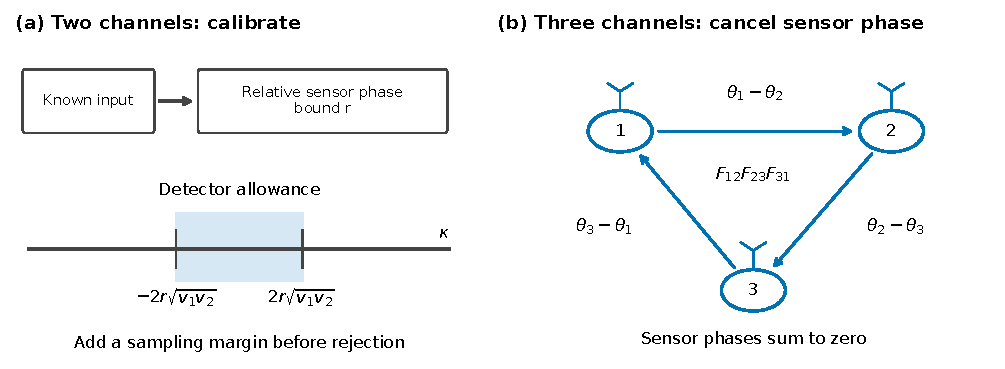
\includegraphics[width=\textwidth]{figures/mechanism_compact.pdf}
\caption{Calibration bounds detector phase, while a three-channel closure product cancels it. The calibrated route allows a nonzero source-null lag contrast and adds a sampling margin. The cycle route uses the three oriented cross spectra; each channel phase appears once with each sign. Both routes still require a full covariance bound. The spectral route also needs a bound on omitted lags.}\label{fig:mechanism}
\end{figure*}

\subsection{A rotating source and the cost of the edge bounds}
Finite detection also requires spectral estimates accurate enough to reveal source motion. We use a three-dimensional version of the trapped-particle model. Random motion relaxes toward the center while a rotational force circulates it about the $(1,1,1)$ axis. The model has
\begin{equation}
 A=\lambda I+\Omega,\quad D=\lambda\Sigma_\xi,\quad
 \Omega=\nu\begin{pmatrix}0&-1&1\\1&0&-1\\-1&1&0\end{pmatrix},
\end{equation}
where $\Sigma_\xi=(1-\xi)I+\xi\mathbf1\mathbf1^{\mathsf T}$. For $\lambda=\log4$ and $\nu=2\pi/(3\sqrt3)$, one sampling interval gives a $2\pi/3$ rotation and a cyclic coordinate permutation, attenuated by $1/4$. The equilibrium control sets $\nu=0$. Both use $\xi=1/4$ and the same family bounds.

Over $0\le\xi\le1/4$ and $\lambda\ge\log4$, the source spectral ceiling is $5/2$. If $g_i$ is the absolute sum of detector coefficients, valid diagonal ceilings are $K_i=(5/2)g_i^2$. Geometric covariance decay also gives the tail allowances at $L=8$ (SM Sec.~S7.3). The filters have principal delays zero, one, and two samples, with small later echoes. These bounds apply to the complete covariance; they are not three independent marginal assertions.

Figure~\ref{fig:study-cycle} shows when these allowances permit rejection. At $N=1048576$, the common and diagonal single-frequency rules each reject $1/200$ rotating records; the two-frequency rule rejects $200/200$. All three reach $200/200$ at $N=2097152$, while equilibrium controls give no rejections. The gain comparison in SM Fig.~S3 explains why diagonal bounds matter: they preserve all $200/200$ rejections across the six transported gains, while a common scalar ceiling loses them at four gains. Valid covariance inflation can also remove detection (SM Fig.~S4).

\begin{figure*}[t]\centering
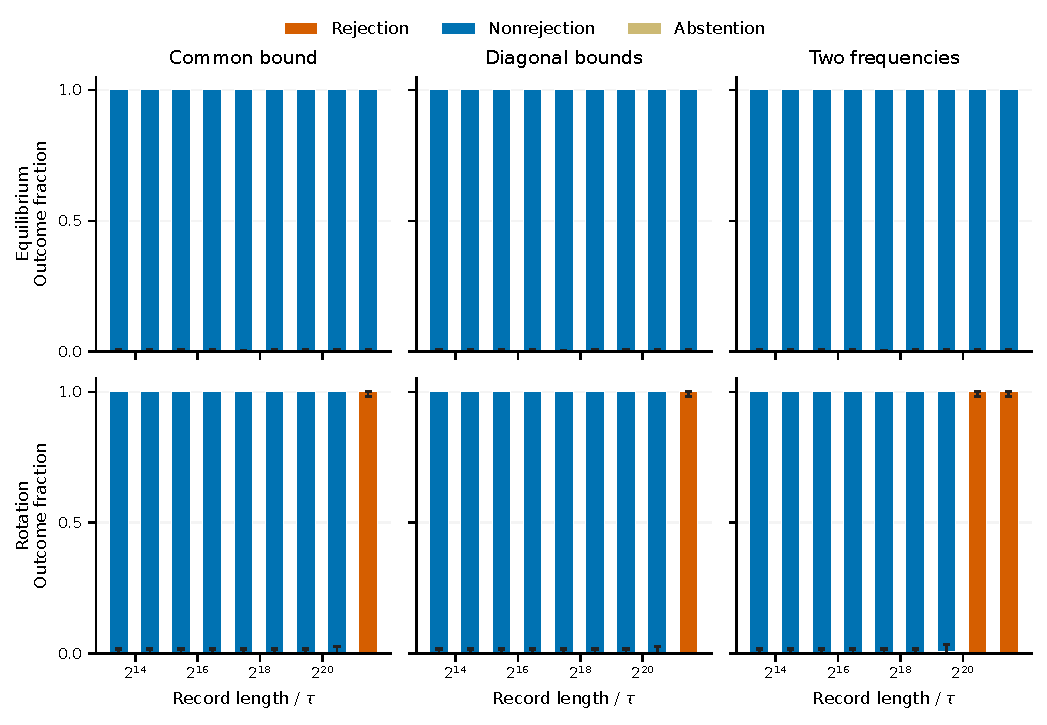
\includegraphics[width=\textwidth]{figures/cycle_operating_compact.pdf}
\caption{The two-frequency rule detects rotation at a shorter tested length than either single-frequency rule. Lengths are shown as $N\log4$ decay times. Fractions use all 200 rotating records per length; equilibrium cells have 400, except 1000 at $N=131072$. Bars are pointwise 95\% binomial intervals. The two-frequency error allowance is included. Common and diagonal decisions coincide in this primary comparison. All methods have zero abstentions. These empirical fractions do not replace the sufficient power condition.}\label{fig:study-cycle}
\end{figure*}
